\documentclass[a4paper,12pt,french]{article}

\usepackage[cours]{../../Style}

\renewcommand{\arraystretch}{1.2}

% Début du document
%%%%%%%%%%%%%%%%%%%
\begin{document}

\title{Variables aléatoires}
\maketitle

\section{Définitions}

\begin{ex}
On lance une pièce équilibrée. Si on tombe sur pile, on gagne 2\euro, sinon on perd 1\euro. On note $X$ les gains après un lancer. Ainsi $X$ peut valoir soit $2$, soit $-1$. La probabilité que $X$ vaille 2, notée $\Pro(X=2)$, vaut $\frac 1 2 = 0,5$. On dit que $X$ est une \textbf{variable aléatoire réelle}.
\end{ex}

\begin{rmqs}
\begin{itemize}
\item Une variable aléatoire réelle est en fait une fonction $X:\Omega \rightarrow \R$: Dans l'exemple précédent, l'univers est $\Omega=\{ \text{\og pile \fg} ; \text{\og face \fg} \}$. On a alors $X( \text{\og pile \fg} ) =2$ et $X( \text{\og face \fg} ) = -1$.

\item En pratique, une variable aléatoire permet de raccourcir les notations: L'évènement \og On gagne 2\euro{} après le lancer \fg devient $X=2$.
\end{itemize}
\end{rmqs}

\rem{Exos \textbf{26},\textbf{27},23 p201 \\
	Exos 48 -> 50 p204}

%\begin{defin}
%Une variable aléatoire réelle est une fonction $X:\Omega \rightarrow \R$
%\end{defin}
%
%\begin{ex}
%Dans l'exemple précédent, on a $\Omega=\{ \text{\og pile \fg} ; \text{\og face \fg} \}$.
%
%On a alors $X( \text{\og pile \fg} ) =2$ et $X( \text{\og face \fg} ) = -1$. 
%\end{ex}

\begin{ex}
\compo[0.6]
{
On reprend l'exemple ci-dessus, mais $X$ représente cette fois les gains après \textbf{deux} lancers successifs. On représente les possibilités grâce à l'arbre ci-contre. On a alors:

\begin{itemize}
\item $\Pro(X=1)=\frac 2 4 = 0,5$ (2 cas favorables sur 4);
\item $\Pro(X=4)=\Pro(X=-2)=\frac 1 4 = 0,25$;
\end{itemize}

On peut alors donner la \textbf{loi de probabilité} de $X$, c'est-à-dire donner la probabilité de chaque issue:

\begin{center}
\begin{tabularx}{0.9\linewidth}{|c|Y|Y|Y|} \hline
$x$ & $-2$ & $1$ & $4$ \\ \hline
$\Pro(X=x)$ & $0,25$ & $0,5$ & $0,25$ \\ \hline
\end{tabularx}
\end{center}

On peut aussi déterminer d'autres probabilités:
\begin{itemize}
\item $\Pro(X \leq 1)=\Pro(X=-2)+\Pro(X=1)=0,75$;
\item $\Pro(X \geq 0) = \Pro(X=1) + \Pro(X=4)=0,75$
\end{itemize}
}
{
\begin{center}
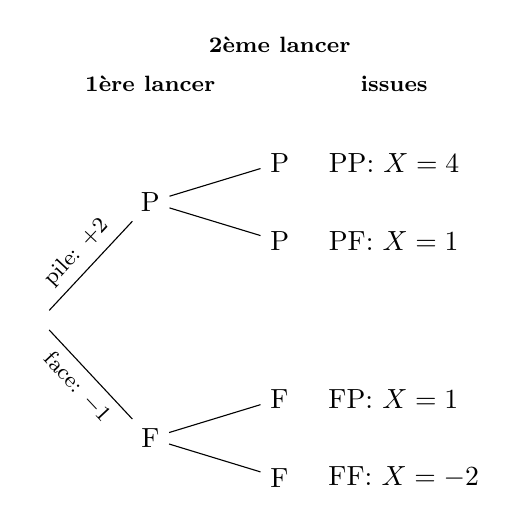
\begin{tikzpicture}[x=1.4cm] % Même effet que xscale=1.8 mais l'option sloped marche

\node (O) at (0,0) {};
\node (P) at (1,1.5) {P};
\node (F) at (1,-1.5) {F};
\node[anchor=west] (PP) at (2,2) {P};
\node[anchor=west] (PF) at (2,1) {P};
\node[anchor=west] (FP) at (2,-1) {F};
\node[anchor=west] (FF) at (2,-2) {F};

\node[right of=PP,anchor=west,node distance=0.5cm] (res) {PP: $X=4$};
\node[right of=PF,anchor=west,node distance=0.5cm] {PF: $X=1$};
\node[right of=FP,anchor=west,node distance=0.5cm] {FP: $X=1$};
\node[right of=FF,anchor=west,node distance=0.5cm] {FF: $X=-2$};

\node[font=\footnotesize\bfseries,above of=P,node distance=1.5cm] (lancer1) {1\up{ère} lancer};
\node[font=\footnotesize\bfseries,above of=PP,node distance=1.5cm] (lancer2) {2\up{ème} lancer};
\node[font=\footnotesize\bfseries,above of=res,node distance=1cm] {issues};

%\draw[->] (lancer1) -- (P);
%\draw[->] (lancer2) -- (PP);

\draw (O) -- (P) node[midway,above,sloped,font=\footnotesize] {pile: $+2$} (P) -- (PP) (P) -- (PF) (O) -- (F) node[midway,below,sloped,font=\footnotesize] {face: $-1$} (F) -- (FP) (F) -- (FF);
\end{tikzpicture}
\end{center}
}
\end{ex}

\rem{Exos \textbf{41},\textbf{43},\textbf{44} p203 \\
	Exos 75 -> 78 p209}

\section{Espérance d'une variable aléatoire}

\begin{defin}
\compo
{
On se donne une variable aléatoire $X$ dont la loi est représentée ci-contre.
}
{
\begin{center}
\begin{tabularx}{0.9\linewidth}{|c|Y|Y|Y|Y|} \hline
$x$ & $x_1$ & $x_2$ & \ldots & $x_N$ \\ \hline
$\Pro(X=x)$ & $p_1$ & $p_2$ & \ldots & $p_N$ \\ \hline
\end{tabularx}
\end{center}
}

\

L'espérance de $X$, notée $\Esp(X)$, est le réel $\Esp(X):=p_1 x_1 + p_2 x_2 + \ldots + p_N x_N$.

Celle-ci représente la moyenne des valeurs de $X$ lorsque l'on répète l'expérience aléatoire un très grand nombre de fois.
\end{defin}

\begin{ex}
On reprend l'exemple ci-dessus. On a $\begin{aligned}[t] \Esp(X) & =0,25 \times (-2) + 0,5 \times 1 + 0,25 \times 4 \\ & = -0,5 + 0,5 + 1 \\ & = 1 \end{aligned}$

L'espérance de $X$ est positive, ce qui veut dire qu'en jouant un grand nombre de fois, le gain moyen par partie sera de 1\euro{} ! Le joueur a donc tout intérêt à faire des parties puisque le jeu est à son avantage.

Évidemment, le jeu restant aléatoire, il est possible (mais très improbable) que le joueur perde dix, cent ou mille parties à la suite et se retrouve ruiné...
\end{ex}

\rem{Exo 28 p201 \\
	Exos 51,53,55,58 p205 \\
	Exos 56,57 p205\\	
	Exox 82,84,86 p215 \\
	Exo 68 p206 \\
	Exo 54 p204 \\
	Sujet D p212}

\section{Expériences à plusieurs épreuves: Cas général}

\begin{fait}
Jusqu'à maintenant, on a répété plusieurs expériences régies par une loi équiprobable. On s'intéresse maintenant à des expériences où chaque issue n'a pas forcément la même probabilité.
\end{fait}

\begin{defin}
Deux évènements sont dits indépendants si la réalisation de l'un n'a aucune influence sur l'autre. La définition s'étend naturellement aux variables aléatoires.
\end{defin}

\begin{ex}
\compo[0.6]
{
On dispose de deux urnes contenant chacune dix boules.
\begin{itemize}
\item La première contient quatre boules rouges (R), trois boules jaunes (J) et trois boules bleues (B).
\item La seconde contient six boules vertes (V) et quatre boules noires (N).
\end{itemize}
Par exemple, la probabilité de tirer une boule rouge dans la première urne est $\frac 4 {10}=0,4$.

On tire \textbf{successivement} une boule de la première puis de la seconde urne.

On représente les issues possibles grâce à l'arbre ci-contre.
}
{
\begin{center}
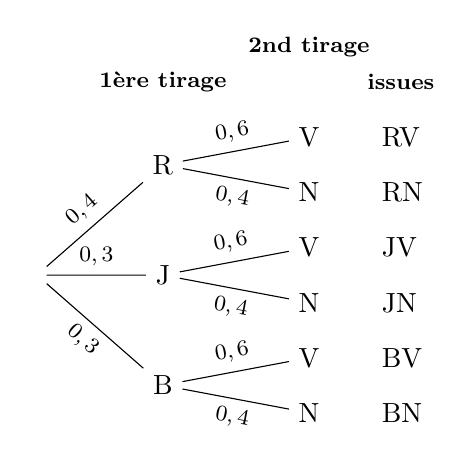
\begin{tikzpicture}[x=1.6cm,y=0.7cm,legende/.style={midway,sloped,font=\footnotesize}] % Même effet que xscale=1.8 mais l'option sloped marche

\node (O) at (0,0) {};
\node (R) at (1,2) {R};
\node (J) at (1,0) {J};
\node (B) at (1,-2) {B};
\node[anchor=west] (RV) at (2,2.5) {V};
\node[anchor=west] (RN) at (2,1.5) {N};
\node[anchor=west] (JV) at (2,0.5) {V};
\node[anchor=west] (JN) at (2,-0.5) {N};
\node[anchor=west] (BV) at (2,-1.5) {V};
\node[anchor=west] (BN) at (2,-2.5) {N};

\node[right of=RV,anchor=west,node distance=0.8cm] (res) {RV};
\node[right of=RN,anchor=west,node distance=0.8cm] {RN};
\node[right of=JV,anchor=west,node distance=0.8cm] {JV};
\node[right of=JN,anchor=west,node distance=0.8cm] {JN};
\node[right of=BV,anchor=west,node distance=0.8cm] {BV};
\node[right of=BN,anchor=west,node distance=0.8cm] {BN};

\node[font=\footnotesize\bfseries,above of=R,node distance=1.05cm] (lancer1) {1\up{ère} tirage};
\node[font=\footnotesize\bfseries,above of=RV,node distance=1.15cm] (lancer2) {2\up{nd} tirage};
\node[font=\footnotesize\bfseries,above of=res,node distance=0.7cm] {issues};

%\draw[->] (lancer1) -- (P);
%\draw[->] (lancer2) -- (PP);

\draw (O) -- (R) node[legende,above] {$0,4$} (R) -- (RV) node[legende,above] {$0,6$} (R) -- (RN) node[legende,below] {$0,4$} (O) -- (J) node[legende,above] {$0,3$} (J) -- (JV) node[legende,above] {$0,6$} (J) -- (JN) node[legende,below] {$0,4$} (O) -- (B) node[legende,below] {$0,3$} (B) -- (BV) node[legende,above] {$0,6$} (B) -- (BN) node[legende,below] {$0,4$};
\end{tikzpicture}
\end{center}
}

\end{ex}

\rem{Exos 30,35,36 p202}

\begin{proprs}
Pour construire et utiliser un arbre de probabilités, on utilisera les règles suivantes:
\begin{itemize}
\item La somme des probabilités inscrites sur les branches issues d'un même nœud est égale à 1;
\item La probabilité d'une issue représentée par un chemin est \textbf{le produit} des probabilités inscrite sur chacune de ses branches;
\item La probabilité d'un évènement est la somme des probabilité de tous les chemins menant à cet évènement.
\end{itemize}
\end{proprs}

\begin{exs}
\begin{itemize}
\item La probabilité d'obtenir une boule rouge puis une boule verte (RV) est $0,4 \times 0,6 = 0,54$.
\item La probabilité d'obtenir une boule autre que rouge puis une boule noire (JV ou BN) est $(0,3 \times 0,6) + (0,3 \times 0,4) = 0,18 + 0,12 = 0,3$.
\end{itemize}
\end{exs}

\rem{Exo 17 p200 \\
	%(Bernoulli) Exos 19 -> 21 p201 \\
	Exos 31,32,33 p202 \\
	Exos 37,38,39 p205 \\
	Exos 67,69,70 p206 \\
	Exo 83 p214 \\
	Exos 71 \rightarrow 74 p209 \\
	Sujets B,C p212}
	
\end{document}